\documentclass{article}
\usepackage{ctex}
\usepackage[xcolor]{listings} % 导入代码高亮包
\usepackage{xcolor} % 导入颜色包
\usepackage{graphicx} % 导入图形包
\author{陈祎伟\\3230102357}
\title{Lab 1: 流水线 RISC-V CPU 设计}
\date{2025年2月24日}

\lstset{
    basicstyle=\ttfamily\footnotesize, % 基本样式,小号等宽字体
    numbers=left,                      % 行号位置
    numberstyle=\tiny\color{gray},     % 行号样式
    stepnumber=1,                      % 行号步长
    numbersep=5pt,                     % 行号与代码间距
    backgroundcolor=\color{white},     % 代码背景色
    showspaces=false,                  % 显示空格
    showstringspaces=false,            % 显示字符串中的空格
    showtabs=false,                    % 显示制表符
    frame=single,                      % 代码框
    rulecolor=\color{black},           % 框颜色
    tabsize=4,                         % 制表符宽度
    captionpos=b,                      % 标题位置
    breaklines=true,                   % 自动换行
    breakatwhitespace=false,           % 仅在空格处换行
    title=\lstname,                    % 显示文件名
    keywordstyle=\color{blue},         % 关键字颜色
    commentstyle=\color{green},        % 注释颜色
    stringstyle=\color{red},           % 字符串颜色
    escapeinside={\%*}{*)},            % 特殊字符
    morekeywords={*,...},              % 额外关键字
    language=[x86masm]Assembler        % 定义asm语言
}

\begin{document}
\maketitle
\section{设计思路}
\subsection{cmp\_32.v文件}
cmp\_32模块用于比较两个32位数的大小关系。\par
实现中,先确定比较关系的类别type(0/1),并得到各个类别下的比较结果res(0/1),type \& res即为最终的比较结果。\par

\subsection{CtrlUnit.v文件}
CtrlUnit模块用于在ID阶段生成各个控制信号。\par
首先将inst\_ID译码得到opcode,funct3以及funct7,进而确定指令类型。再由指令类型确定各控制信号,部分信号如下:\par
\begin{itemize}
    \item Branch信号:Branch信号用于指示是否需要跳转,即符合条件的branch指令以及jal与jalr指令。\par
\begin{lstlisting}[language=Verilog]
    assign Branch = (B_valid & cmp_res) | JAL | JALR;
\end{lstlisting}
    \item cmp\_ctrl信号:根据指令类型确定比较控制信号,传输给cmp\_32模块。\par
    \item ALUSrc信号:根据指令类型确定ALU的输入数据来源,传输给ALU模块。\par
    \subitem{1} ALUSrc\_A信号:指示ALU操作数A的来源,为rs1或者PC。\par
\begin{lstlisting}[language=Verilog]
        assign ALUSrc_A = JAL | JALR | AUIPC;
\end{lstlisting}
    \subitem{2} ALUSrc\_B信号:指示ALU操作数B的来源,为rs2或者立即数。\par
\begin{lstlisting}[language=Verilog]
        assign ALUSrc_B = I_valid | L_valid | S_valid | AUIPC | LUI | JAL | JALR;
\end{lstlisting}
    \item rs\_use信号:指示rs1和rs2是否被使用,即ALUSrc信号取反:\par
\begin{lstlisting}[language=Verilog]
    assign rs1use = ~ALUSrc_A;
    assign rs2use = ~ALUSrc_B;  
\end{lstlisting} 
    \item hazard\_optype信号:指示当前指令的类型,用于冒险检测。\par
    其中识别了四种类型:Branch、S\_valid、L\_valid、其他,分别对应11、10、01、00。
\begin{lstlisting}[language=Verilog]
    assign hazard_optype = Branch ? 2'b11 :
                           S_valid ? 2'b10 :
                           L_valid ? 2'b01 :
                           2'b00; 
\end{lstlisting}
\end{itemize}

\subsection{HazardDetectionUnit.v文件}
HazardDetectionUnit模块主要接收了ID、EX、MEM阶段的寄存器使用情况以及CtrlUnit模块产生的hazard\_optype信号,从而产生各forwarding控制信号以及流水线寄存器的控制信号,具体实现如下:\par
\begin{enumerate}
    \item 首先定义寄存器hazard\_optype\_EXE、hazard\_optype\_MEM,传递存储接收的hazard\_optype\_ID信号:\par
\begin{lstlisting}[language=Verilog]
    reg [1:0] hazard_optype_EXE, hazard_optype_MEM;
    initial begin
        hazard_optype_EXE = 2'b00;
        hazard_optype_MEM = 2'b00;
    end
    always @(posedge clk) begin
        hazard_optype_EXE <= hazard_optype_ID;
        hazard_optype_MEM <= hazard_optype_EXE;
    end
\end{lstlisting}
    \item 利用hazard\_optype选择各条forwarding路径:\par
    其中,一般的forwarding路径分为3条,分别对应EX-\textgreater{}ID、EX\_MEM-\textgreater{}ID、MEM-\textgreater{}ID;\par
    而为了处理load-store类型的hazard,另外添加了一条forwarding路径,即MEM-\textgreater{}EXE来避免stall,具体实现如下:\par
\begin{lstlisting}[language=Verilog]
    assign forward_ctrl_A = rs1use_ID ? rd_EXE == rs1_ID \
                       && rd_EXE != 5'b0 ? 2'b01 :
              rd_MEM == rs1_ID && rd_MEM != 5'b0 ? \
              hazard_optype_MEM == 2'b01 ? 2'b11 :
                            2'b10 : 2'b00 : 2'b00;
    assign forward_ctrl_B = rs2use_ID ? rd_EXE == rs2_ID \
                       && rd_EXE != 5'b0 ? 2'b01 :
              rd_MEM == rs2_ID && rd_MEM != 5'b0 ? \
              hazard_optype_MEM == 2'b01 ? 2'b11 :
                            2'b10 : 2'b00 : 2'b00;

    assign forward_ctrl_ls = hazard_optype_EXE == 2'b10 && \
        hazard_optype_MEM == 2'b01 && rd_MEM == rs2_EXE && \
                                rd_MEM != 5'b0 ? 1'b1 : 1'b0;
\end{lstlisting}

    \item 判断是否需要stall、类型以及处理:\par
    先定义load\_use\_hazard信号以及control\_hazard信号:
\begin{lstlisting}[language=Verilog]
    wire load_use_hazard = hazard_optype_EXE == 2'b01 && (rd_EXE == rs1_ID || rd_EXE == rs2_ID) && rd_EXE != 5'b0 && hazard_optype_ID != 2'b10 ? 1'b1 : 1'b0;
    wire branch_hazard = hazard_optype_ID == 2'b11 ? 1'b1 : 1'b0;
\end{lstlisting}
    对于两种不同的stall类型,分别对流水线寄存器进行控制:
\begin{lstlisting}[language=Verilog]
    assign PC_EN_IF = load_use_hazard ? 1'b0 : 1'b1;
    assign reg_FD_stall = load_use_hazard ? 1'b1 : 1'b0;
    assign reg_FD_flush = branch_hazard ? 1'b1 : 1'b0;
    assign reg_DE_flush = load_use_hazard ? 1'b1 : 1'b0;                                                      

    assign reg_EM_flush = 1'b0;
    assign reg_FD_EN = 1'b1;
    assign reg_DE_EN = 1'b1;
    assign reg_EM_EN = 1'b1;
    assign reg_MW_EN = 1'b1;
\end{lstlisting}
\end{enumerate}

\subsection{RV32core.v文件}
在RV32core模块中,按序传输上述各阶段的信号,实现流水线的控制。部分实现如下:\par
\begin{lstlisting}[language=Verilog]
    ...
    MUX2T1_32 mux_IF(.I0(PC_4_IF),.I1(jump_PC_ID),.s(Branch_ctrl),.o(next_PC_IF)); // choose next PC according to the control signal
    ...
    MUX4T1_32 mux_forward_A(.I0(rs1_data_reg),.I1(ALUout_EXE),.I2(Dataout_MEM),.I3(Datain_MEM), 
        .s(forward_ctrl_A),.o(rs1_data_ID));
    MUX4T1_32 mux_forward_B(.I0(rs2_data_reg),.I1(ALUout_EXE),.I2(Dataout_MEM),.I3(Datain_MEM),
        .s(forward_ctrl_B),.o(rs2_data_ID)); // select the ALU's operand according to the forward_ctrl signal, realize forwarding

    MUX2T1_32 mux_forward_EXE(.I0(rs2_data_EXE),.I1(Datain_MEM),.s(forward_ctrl_ls),.o(Dataout_EXE)); // forward_ctrl_ls signal controls load-store forwarding
\end{lstlisting}

\section{思考题}
\subsection{添加了 Forwarding 机制后,是否观察到了 stall 延迟减少的情况?请在测试程序中给出 Forwarding 机制起到实际作用的位置,并给出仿真图加以证明。(只需要贴出一次 Forwarding 机制起效的仿真图片即可)}

~\par
添加了forwarding机制之后,各条forwarding路径均带来了一定的stall延迟减少。\par

例如load-store的forwarding路径,相对于一般的load-use hazard处理方式(stall一周期 + forwarding),每次可以减少一个周期的stall;而相对于没有任何forwarding优化的情况,可以减少2个周期的stall。

测试程序中PC=F8处出现了load-store类型:
\begin{verbatim}
    ...
    lw   x8, 24(x0) # PC = 0xF8, x8 = 0xFF000F0F
    sw   x8, 28(x0) # PC = 0xFC
    lw   x1, 28(x0) # PC = 0x100, x1 = 0xFF000F0F
    ...
\end{verbatim}

\begin{figure}[h]
    \centering
    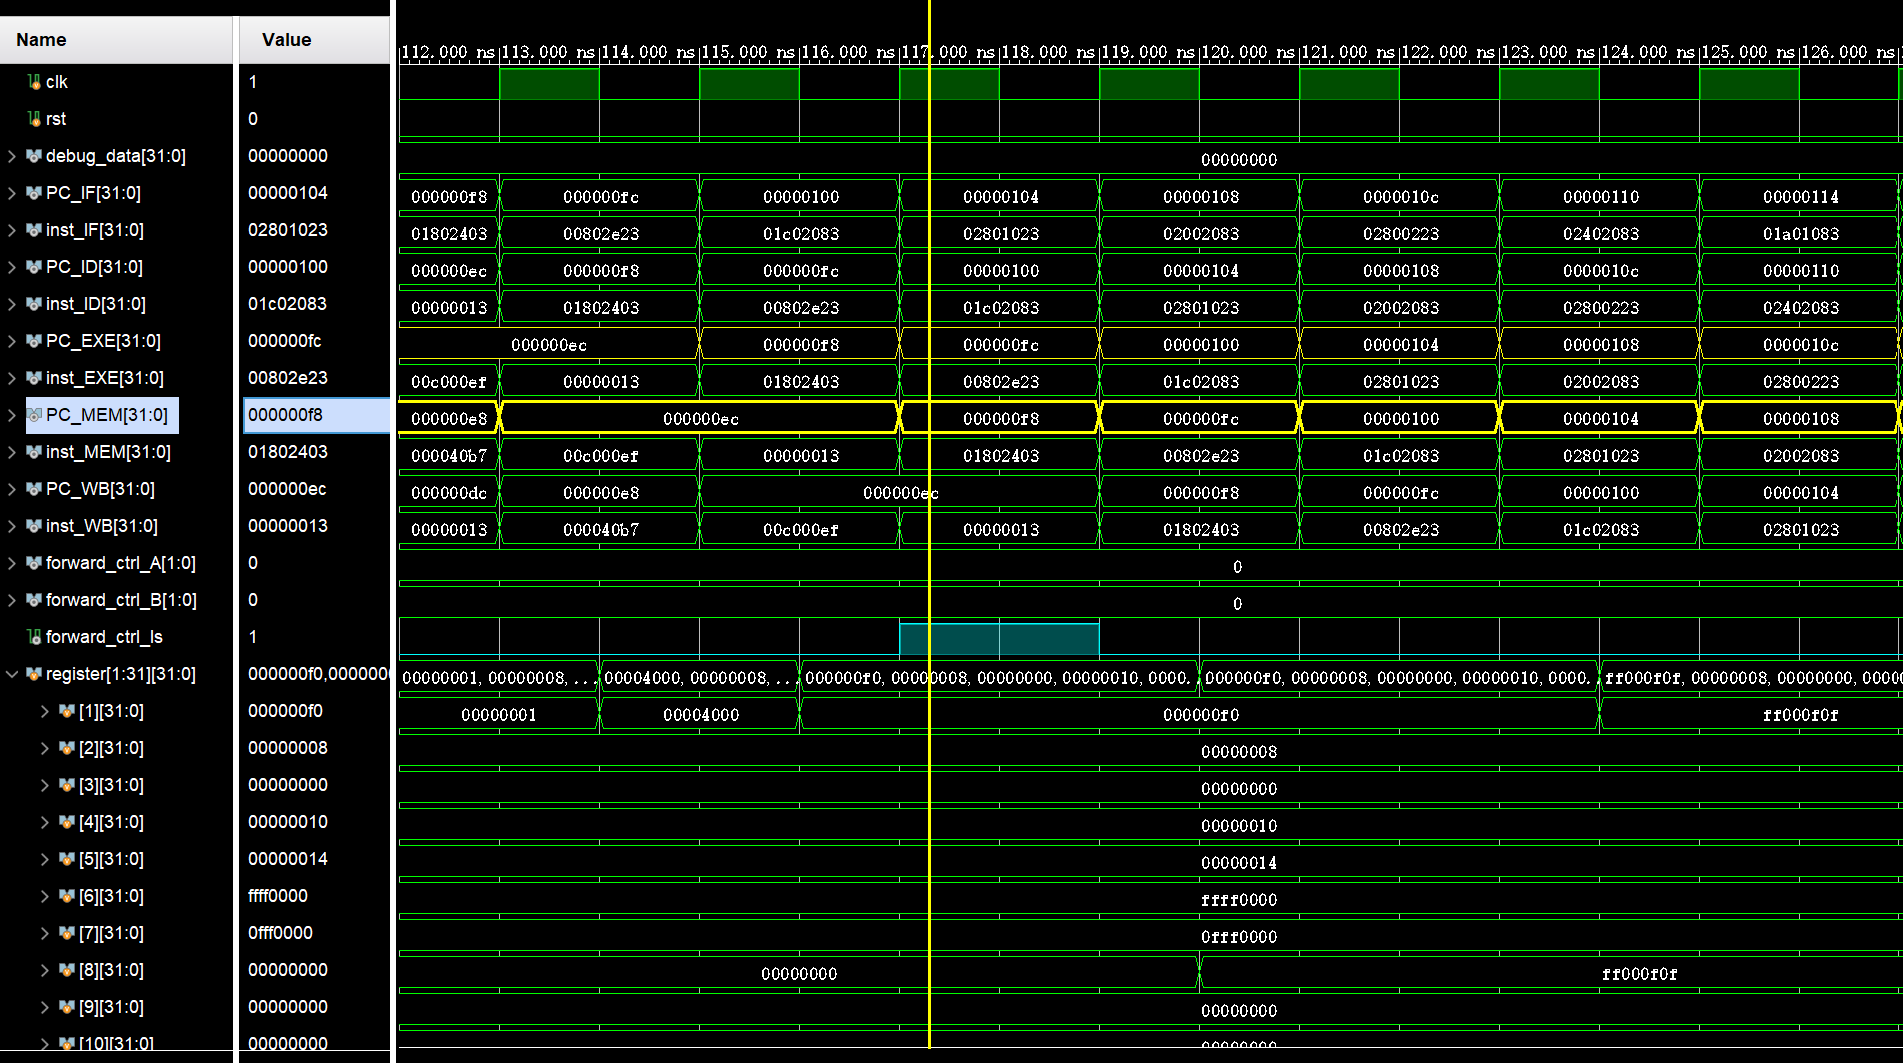
\includegraphics[width=1.2\textwidth]{ls.png}
    \caption{Load-Store Forwarding Example}
    \label{fig:ls}
\end{figure}

图1中可见,当lw x8, 24(x0)执行到MEM阶段,sw x8, 28(x0)执行到EX阶段时,forward\_ctrl\_ls信号拉高,load-store的forwarding路径启动。\par
下一个周期,x8寄存器被正常写入数据,且第3条指令lw x1, 28(x0)紧接着正常执行,并未出现stall;最终x1寄存器被正常写入数据0xFF000F0F。\par
由此,load-store的forwarding路径成功减少了stall 延迟。

\newpage
\subsection{在我们的框架中,比较器 cmp\_32 处于 ID 段。请说明比较器在 ID 对比比较器在 EX 的优劣。(提示:可以从时延的角度考虑)}

~\par
\begin{itemize}
    \item 优势:比较器位于ID阶段,可以缩短分支跳转指令的时延。
    如果比较器位于EX阶段,则branch指令的跳转判断被滞后。\par
    当不发生跳转时,比较器位于ID阶段的设计不需要额外的stall,而位于EX阶段需要一个周期的stall;\par
    当发生跳转时,比较器位于ID阶段的设计需要一个周期的stall,而位于EX阶段需要两个周期的stall;\par
    可见比较器位于ID阶段缩短了分支跳转指令的时延。

    \item 劣势:比较器位于ID阶段,可能打破流水线各个阶段的相对平衡,增大ID阶段的负担,增加时延。
    \item 总体而言,对于分支跳转指令较多的情境下,比较器位于ID阶段的设计会显现出更大的优势;而当分支跳转指令较少的情况下,二者性能还需比较。
\end{itemize}
\end{document}
